\chapter{Results and Discussion} % Main chapter title

\label{Chapter5} % Change X to a consecutive number; for referencing this chapter elsewhere, use \ref{ChapterX}

\section{Phenanthrene Parameterization}


\section{Solvation free energies}

The force field parameters for phenanthrene were estimated as described above and the ones for the other compounds were retrieved from the literature \cite{lobanova2016,herdes2015,ervik2016,muller2017}:
alifaticos
\begin{table*}[h]
\centering
  \caption{SAFT-$\gamma$ Mie Force Field for each substance used in this work}
  \label{tbl:parameters}
  \begin{tabular}{lllll}
  	\hline
  	               & $m_s$ & $\epsilon/k_{B}$ (K) & $\sigma (\dot{A})$ & $\lambda_r$ \\ \hline
  	Water          & 1     & 305.21               & 2.902              & 8.0         \\
  	Propane        & 1     & 426.08               & 4.871              & 34.29       \\
  	Carbon dioxide & 2     & 194.94               & 2.848              & 14.65       \\
  	Hexane         & 2     & 376.35               & 4.508              & 19.57       \\
  	Octanol        & 3     & 495.71               & 4.341              & 28.79       \\
  	Toluene        & 3     & 268.24               & 3.685              & 11.80       \\
  	Benzene        & 3     & 230.30               & 3.441              & 10.45       \\
  	Pyrene         & 4     & 459.04               & 4.134              & 15.79       \\
  	Anthracene     & 5     & 259.68               & 3.631              & 9.55        \\
  	Phenanthrene   & 5     & 262.74               & 4.077              & 9.55        \\ \hline
  \end{tabular}

\end{table*}

\begin{table*}[h]
\centering
  \caption{Calculated and experimental values for solvation free energies (kcal/mol) of solutes in non aqueous solvents}
  \label{tbl:solv1}
  \begin{tabular}{lllll}
    \hline
      Solvent & Solute & $\Delta G_{solv}^{exp}$ & $\Delta G_{solv}^{Mie}$ & Absolute \\
      & & & &Deviation \\
    \hline
    hexane    & benzene      & -3.96  & -3.76  $\pm$ 0.01 & 0.20 \\
    hexane    & pyrene       & -11.53 & -10.82 $\pm$ 0.02 & 0.71 \\
    hexane    & phenanthrene & -10.01 & -9.16  $\pm$ 0.01 & 0.85 \\
    toluene   & pyrene       & -12.86 & -11.74 $\pm$ 0.01 & 1.11\\
    toluene   & anthracene   & -11.31 & -9.90 $\pm$ 0.01 & 1.41\\
    1-octanol & propane      & -1.32  & -1.36  $\pm$ 0.02 & 0.04 \\
    1-octanol & anthracene   & -11.72 & -8.16  $\pm$ 0.03 & 3.61 \\
    1-octanol & phenanthrene & -10.22 & -8.34  $\pm$ 0.03 & 1.47 \\
    \hline
    RMSE      &              &        &                   & 1.48     \\
    \hline
  \end{tabular}
\end{table*}

\begin{figure}
\centering
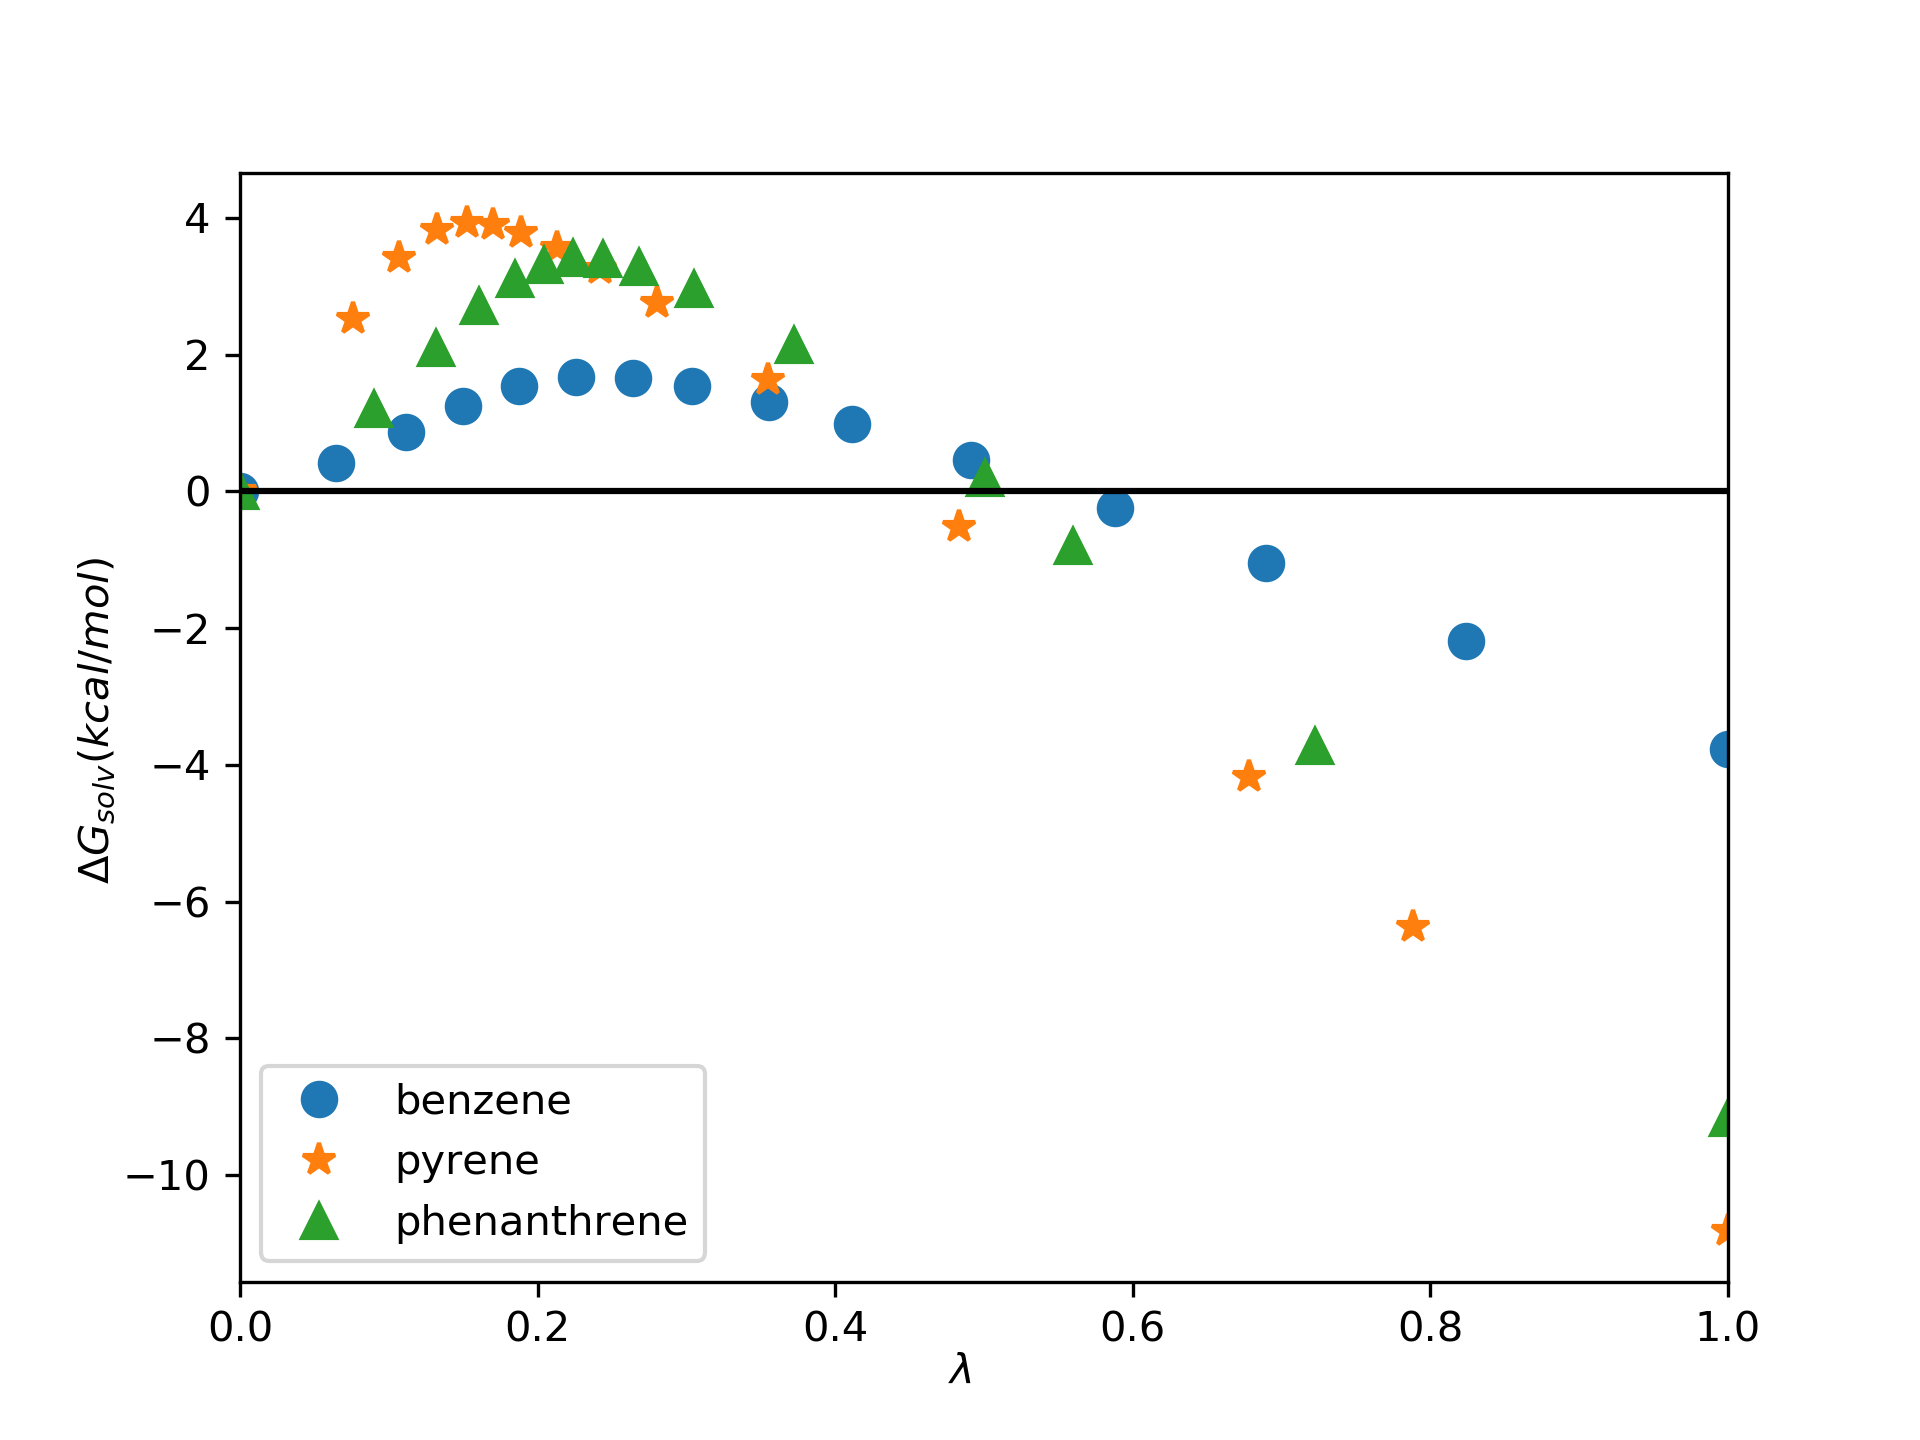
\includegraphics[width=0.9\linewidth]{Figures/hex}
\caption{Solvation free energy profiles for the hexane solvent}
\label{fig:hex}
\end{figure}

\begin{figure}
	\centering
    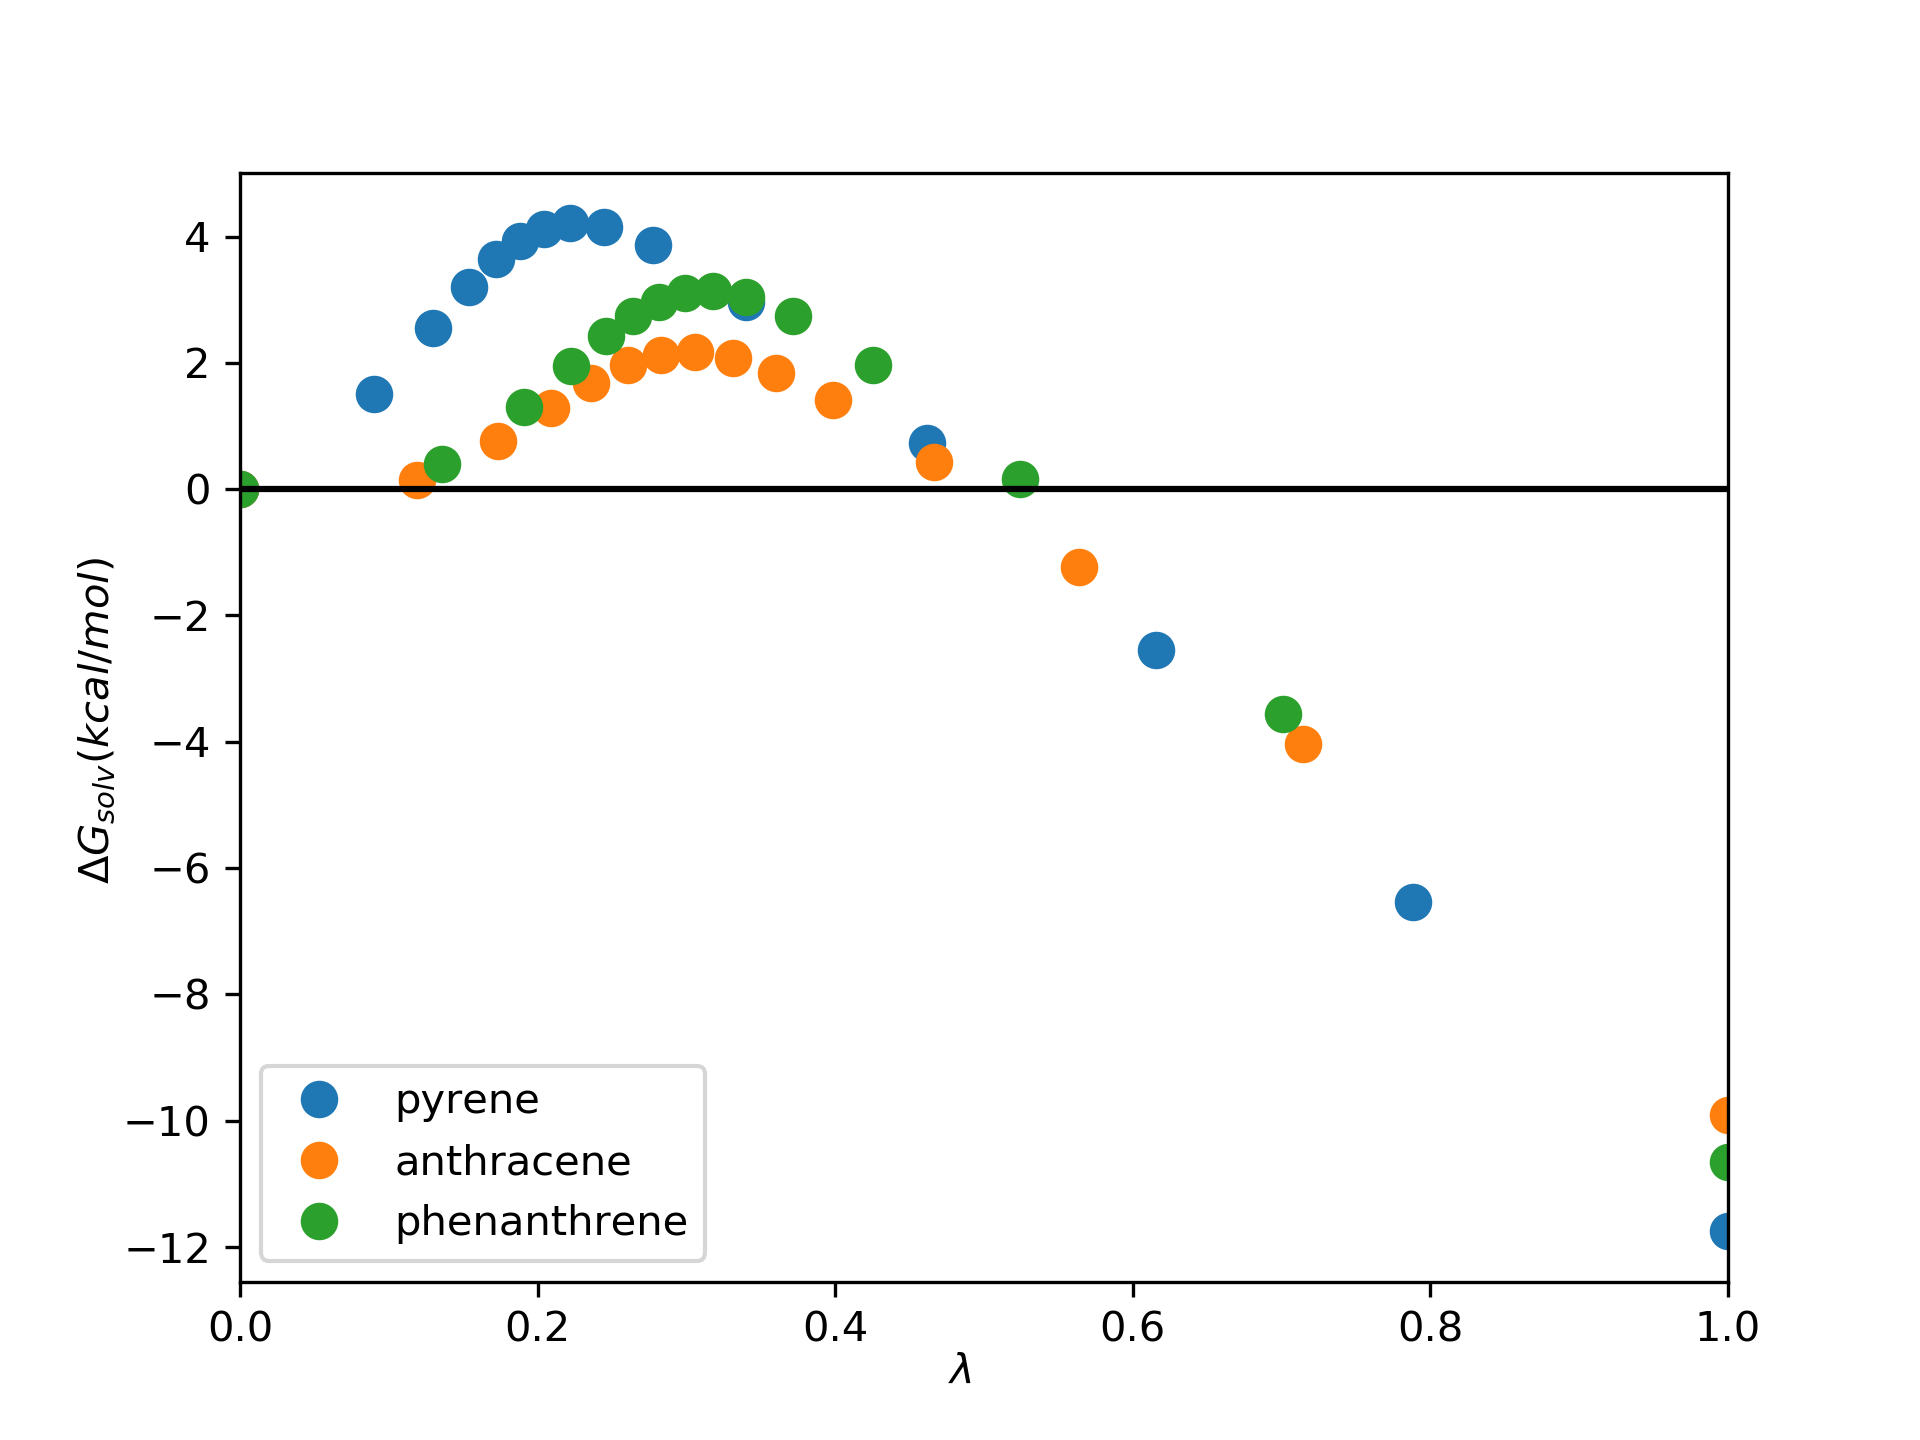
\includegraphics[width=0.9\linewidth]{Figures/tol}
    \caption{Solvation free energy profiles for the toluene solvent }
    \label{fig:tol}
\end{figure}

\begin{figure}
\centering
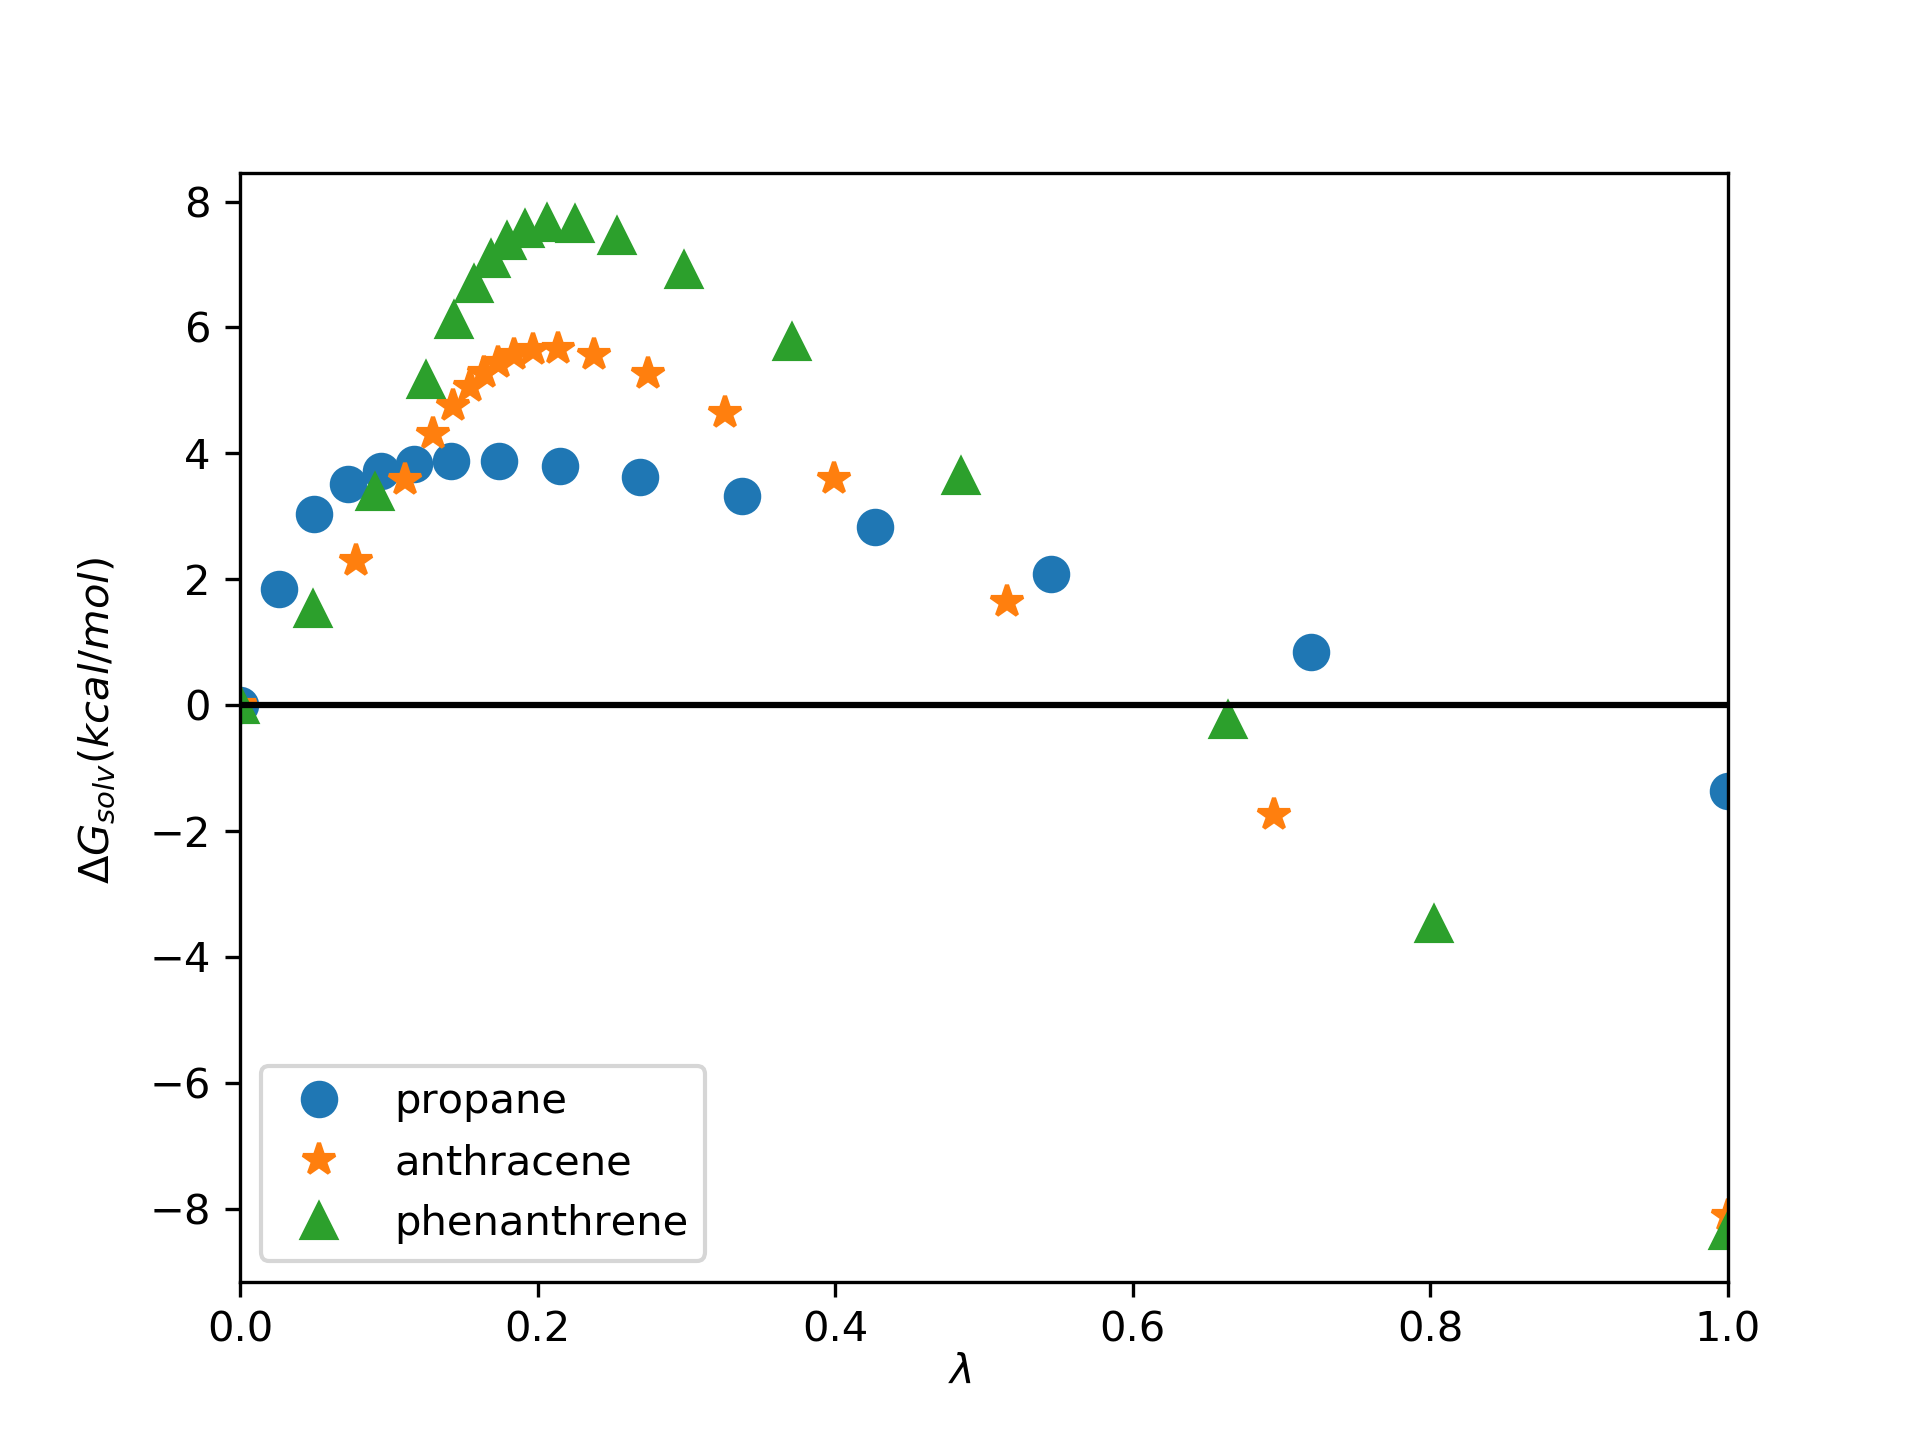
\includegraphics[width=0.9\linewidth]{Figures/oct}
\caption{Solvation free energy profiles for the 1-octanol solvent}
\label{fig:oct}
\end{figure}

\FloatBarrier
\begin{table}[H]
\centering
  \caption{Calculated values for the solvation free energies (kcal/mol) of phenanthrene in toluene+$CO_{2}$}
  \label{tbl:solv3}
  \begin{tabular}{ll}
    \hline
      $w_{CO_{2}}$ & $\Delta G_{solv}^{Mie}$ \\
    \hline
    0.0    & -10.65 $\pm$ 0.02   \\
    0.087  & -10.73 $\pm$ 0.02   \\
    0.119  & -10.78 $\pm$ 0.02   \\
    0.169  & -10.71 $\pm$ 0.02   \\
    0.289  & -10.69 $\pm$ 0.02   \\
    \hline
  \end{tabular}
\end{table}
\FloatBarrier

\begin{figure}[H]
\centering
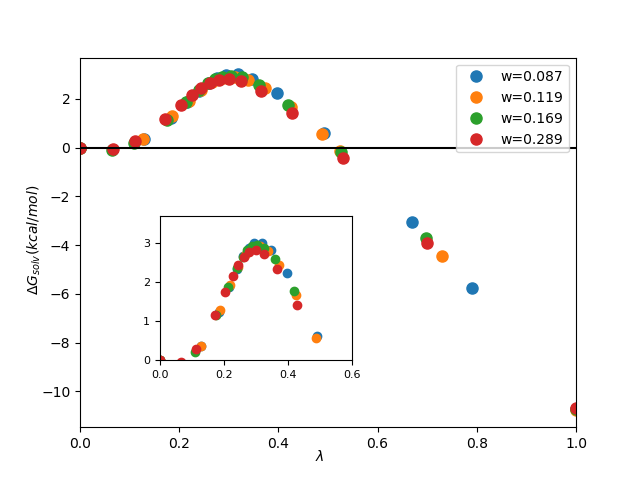
\includegraphics[width=0.9\linewidth]{Figures/Figure_1}
\caption{Solvation free energy profiles of phenanthrene in toluene+$CO_{2}$}
\label{fig:Figure_1}
\end{figure}


\section{Hydration free energies}

\begin{table*}[h]
	\centering
	\caption{Calculated values for the Gibbs energy of solvation (kcal/mol) of solutes in water for $k_{ij}=0$}
	\label{tbl:solv3}
	\begin{tabular}{ll}
		\hline
		Solute & $\Delta G_{solv}^{Mie}$ \\
		\hline
		propane   & 1.10 $\pm$ 0.01   \\
		benzene  & -4.45 $\pm$ 0.03   \\
		toluene  & -15.80 $\pm$ 0.06   \\
		phenanthrene & -10.90 $\pm$ 0.04   \\
		\hline
	\end{tabular}
\end{table*}
\begin{table*}[h]
  \centering
  \caption{Binary interaction parameters employed}
  \label{tbl:kij}
  \begin{tabular}{ll}
    \hline
      Pair & $k_{ij}$ \\
    \hline
    water  + propane      & 0.067  \\
    water  + aromatic      & 0.154 \\  
    \hline
  \end{tabular}
\end{table*}

\begin{table*}[!htb]
  \centering
  \caption{Calculated and experimental values for the Gibbs energy of solvation (kcal/mol) of solutes in water}
  \label{tbl:solv2}
  \begin{tabular}{lllll}
    \hline
     Solute      & $\Delta G_{solv}^{exp}$ & $\Delta G_{solv}^{Mie}$ & Absolute Deviation &$\Delta G_{solv}^{GAFF}$ \\
    \hline
    propane      &  2.00 $\pm$ 0.20 & 2.01 $\pm$ 0.01& 0.01 &2.50 $\pm$0.02 \\
    benzene      & -0.86 $\pm$ 0.20 & -1.12 $\pm$ 0.01    &  0.26    &-0.81$\pm$0.02 \\  
    toluene      & -0.83 $\pm$ 0.20 & -0.84 $\pm$ 0.01   &  0.01    &-0.79$\pm$0.03\\
    phenanthrene & -3.88 $\pm$ 0.60 & 3.47 $\pm$ 0.02& 0.41 &-5.26$\pm$0.03 \\
    \hline
    RMSE         &                  &               &  0.24     &      \\
    \hline
  \end{tabular}

\end{table*}


\begin{figure}
\centering
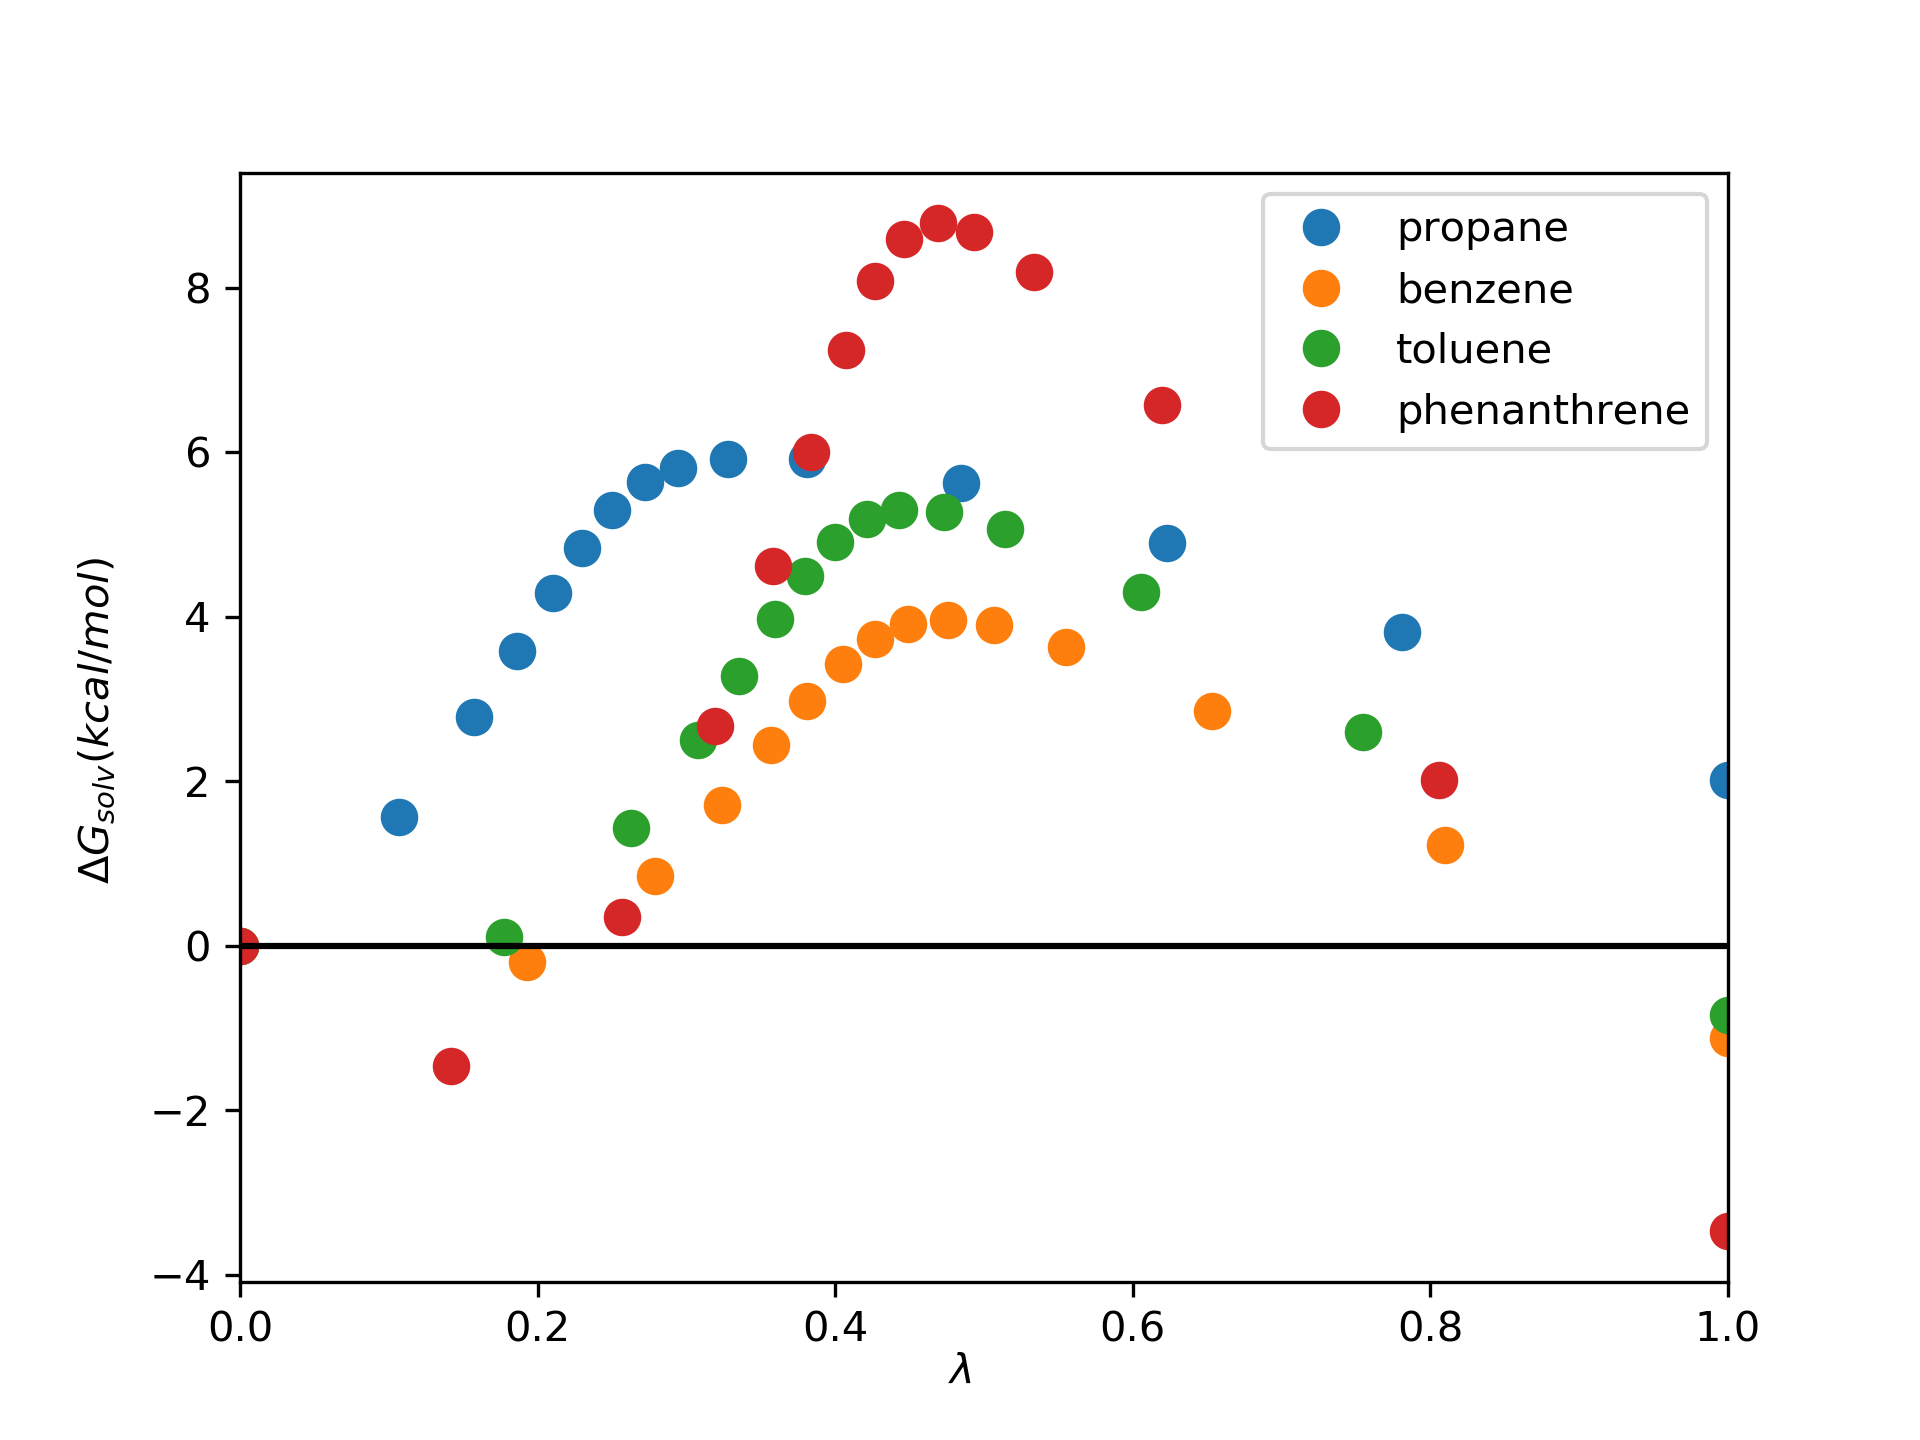
\includegraphics[width=0.9\textwidth]{Figures/water}
\caption{Hydration free energy profiles}
\label{fig:water}
\end{figure}

